\let\negmedspace\undefined
\let\negthickspace\undefined
\documentclass[journal]{IEEEtran}
\usepackage[a5paper, margin=10mm, onecolumn]{geometry}
%\usepackage{lmodern} % Ensure lmodern is loaded for pdflatex
\usepackage{tfrupee} % Include tfrupee package

\setlength{\headheight}{1cm} % Set the height of the header box
\setlength{\headsep}{0mm}     % Set the distance between the header box and the top of the text

\usepackage{gvv-book}
\usepackage{gvv}
\usepackage{cite}
\usepackage{amsmath,amssymb,amsfonts,amsthm}
\usepackage{algorithmic}
\usepackage{graphicx}
\usepackage{textcomp}
\usepackage{xcolor}
\usepackage{txfonts}
\usepackage{listings}
\usepackage{enumitem}
\usepackage{mathtools}
\usepackage{gensymb}
\usepackage{comment}
\usepackage[breaklinks=true]{hyperref}
\usepackage{tkz-euclide} 
\usepackage{listings}
% \usepackage{gvv}                                        
\def\inputGnumericTable{}                                 
\usepackage[latin1]{inputenc}                                
\usepackage{color}                                            
\usepackage{array}                                            
\usepackage{longtable}                                       
\usepackage{calc}                                             
\usepackage{multirow}                                         
\usepackage{hhline}                                           
\usepackage{ifthen}                                           
\usepackage{lscape}
\usepackage{xr}
\externaldocument{/home/homa/Desktop/matgeo/main}
\begin{document}

\bibliographystyle{IEEEtran}
\vspace{3cm}

\title{3-3.3-8}
\author{EE24BTECH11062 - Homa Harshitha Vuddanti
}
% \maketitle
% \newpage
% \bigskip
{\let\newpage\relax\maketitle}

\renewcommand{\thefigure}{\theenumi}
\renewcommand{\thetable}{\theenumi}
\setlength{\intextsep}{10pt} % Space between text and floats


\numberwithin{equation}{enumi}
\numberwithin{figure}{enumi}
\renewcommand{\thetable}{\theenumi}


\textbf{Question}:\\
Construct a triangle $ABC$ with side $BC = 7 cm, \angle{B}=45\degree , \angle{A}=105\degree$.   
\\
\textbf{Solution: }\\
Given,\\
\begin{table}[h!]    
  \centering
  \begin{tabular}[12pt]{ |c| c|}
    \hline
    \textbf{Variable} & \textbf{Description}\\ 
    \hline
    $a$ & $7cm$\\
    \hline 
    $\angle{B}$ & $45\degree$\\
    \hline
    $\angle{A}$ & $105\degree$\\
    \hline
    \end{tabular}




  \caption{Given variables}
  \label{3-3.3-8-table}
\end{table}

By angle sum property,
\begin{align}
    \angle{A}+\angle{B}+\angle{C}&=\pi\\
    \angle{C}&=\pi-\brak{\frac{\pi}{4}+\frac{7\pi}{12}}\\
    \angle{C}&=\frac{\pi}{6}\label{3-3.3-8-1}
\end{align}
Using projection rule,
\begin{align}
    a&=b \cos C+c \cos B\\
    b\cos C+c\cos B-a&=0\label{3-3.3-8-2}
\end{align}
Using Sine formula, in $\triangle ABC$,
\begin{align}
    \frac{a}{sin A}=\frac{b}{sin B}=\frac{c}{sin C}
\end{align}
 \begin{align}
    b\sin C&= c\sin B\\
    b\sin C - c\sin B &=0\label{3-3.3-8-3}
\end{align}
 Solving equations \eqref{3-3.3-8-2}and \eqref{3-3.3-8-3},
\begin{align}
\myvec{\cos C && \cos B\\ \sin C && -\sin B}\myvec{b \\ c}=\myvec{a \\ 0}\\
\myvec{\cos \frac{\pi}{6} && \cos \frac{\pi}{4}\\ \sin \frac{\pi}{6} && -\sin\frac{\pi}{4}}\myvec{b \\ c}=\myvec{7 \\ 0}\\
\myvec{\frac{\sqrt{3}}{2} && \frac{1}{\sqrt{2}}\\ \frac{1}{2} && -\frac{1}{\sqrt{2}}}\myvec{b \\ c}=\myvec{7 \\ 0}
\end{align}
Solving for $b$ and $c$,
\begin{align}
    \myvec{\frac{\sqrt{3}}{2} && \frac{1}{\sqrt{2}} && 7 \\ \frac{1}{2} && -\frac{1}{\sqrt{2}} && 0}\xrightarrow{R1=R1+R2}\myvec{\frac{\sqrt{3}+1}{2} && 0 && 7 \\ \frac{1}{2} && -\frac{1}{\sqrt{2}} && 0}\xrightarrow{R2=\frac{R1}{\sqrt{3}+1}-R2}\\\myvec{\frac{\sqrt{3}+1}{2} && 0 && 7 \\ 0 && \frac{1}{\sqrt{2}} && \frac{7}{\sqrt{3}+1}}\xrightarrow{R1=\frac{2}{\sqrt{3}+1}R1, R2=\sqrt{2}R2}\myvec{1 && 0 && \frac{14}{\sqrt{3}+1} \\ 0 && 1 && \frac{7\sqrt{2}}{\sqrt{3}+1}}
\end{align}
\begin{align}
    b&=\frac{14}{\sqrt{3}+1}\\
    c&=\frac{7\sqrt{2}}{\sqrt{3}+1}
\end{align}
 From \eqref{eq:9/11/2/1},
 \begin{align}
 \vec{A}&=c\myvec{\cos B\\ \sin B}=\myvec{\frac{7}{\sqrt{3}+1} \\ \frac{7}{\sqrt{3}+1}}\\
\vec{B}&=0\\
\vec{C}&=\myvec{a \\ 0}=\myvec{7\\0}
 \end{align}
\begin{figure}[h!]
   \centering
   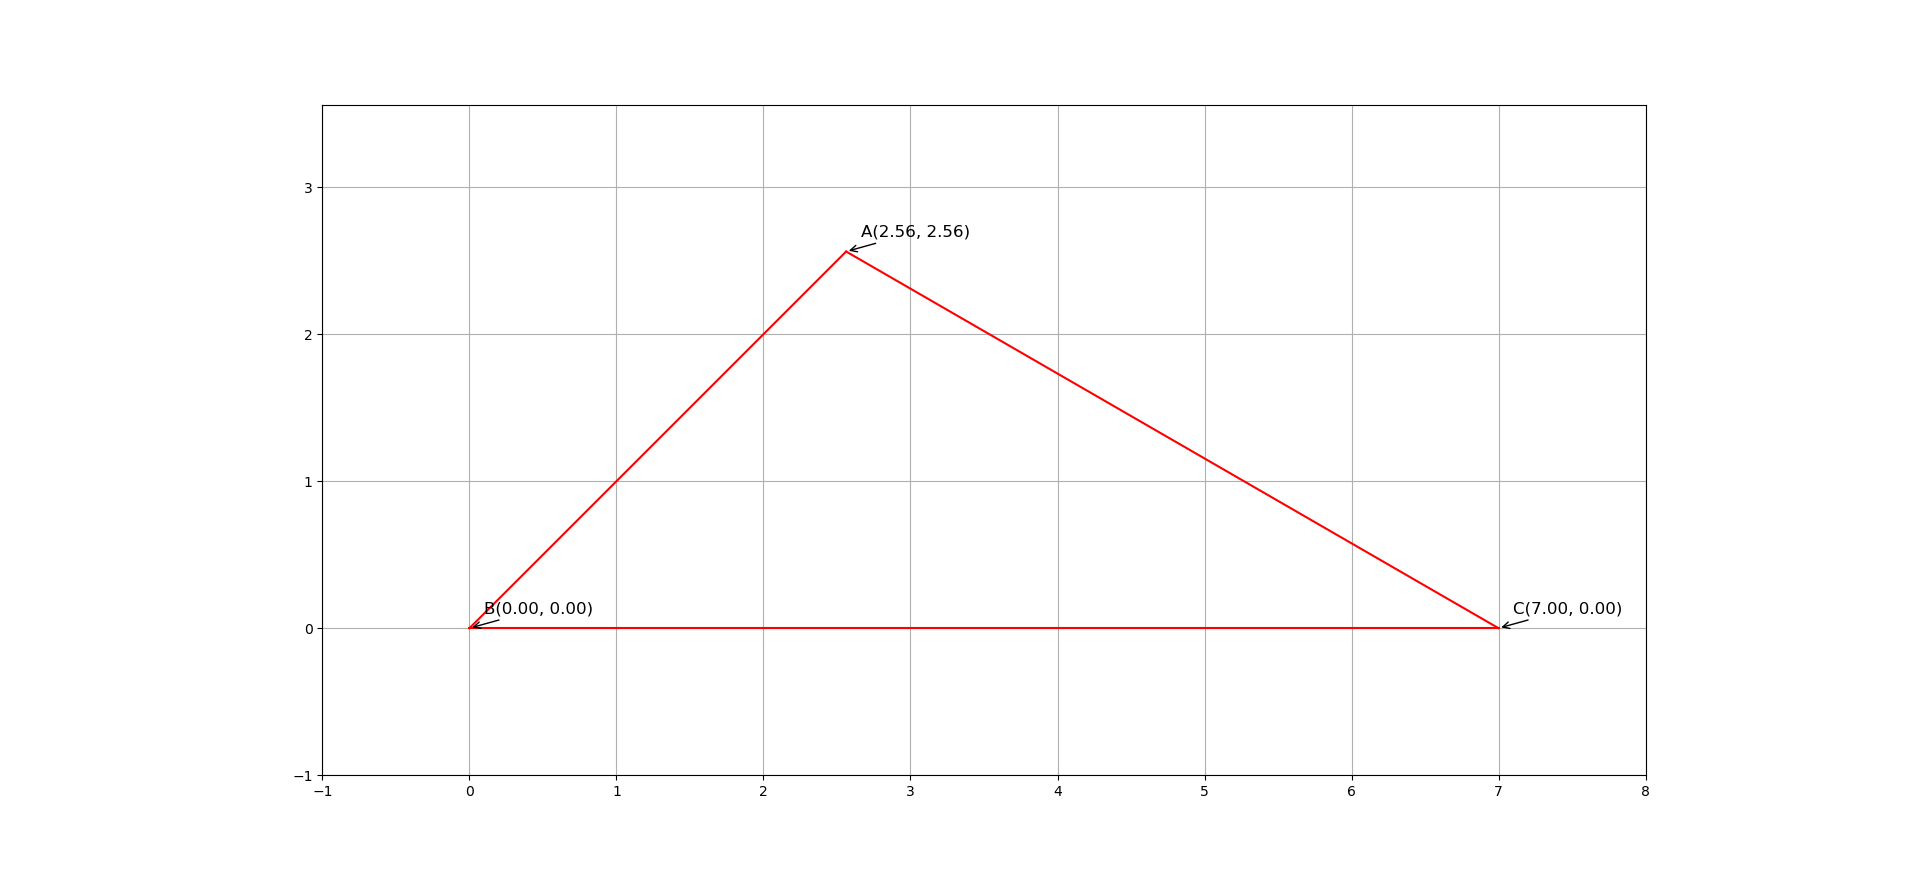
\includegraphics[width=1.1\columnwidth]{Figs/Figure_1.png}
   \caption{Plot}
   \label{3-3.3-8-Figure}
\end{figure}
\end{document}  






